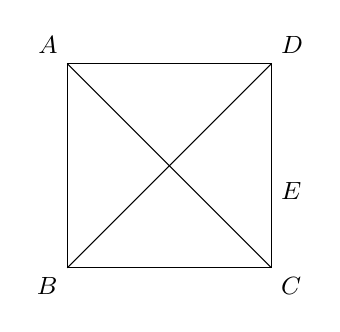
\begin{tikzpicture}[scale=.72, every node/.style={font=\small}]
  \coordinate (A) at (0,3.6); \coordinate (B) at (0,0);
  \coordinate (C) at (3.6,0); \coordinate (D) at (3.6,3.6); \coordinate (E) at (3.6,1.35);
  \draw (A)--(B)--(C)--(D)--cycle; \draw (A)--(C); \draw (B)--(D);
  \foreach \p/\pos in {A/above left,B/below left,C/below right,D/above right,E/right}
    \node[\pos] at (\p) {$\p$};
\end{tikzpicture}
